% Fig. 4 -- ownership (column width, Section 6)
\begin{figure}[htbp]
  \centering
  \subcaptionbox{Tool-boundary result ownership and the lifetime of a shared object\label{fig:designs}}{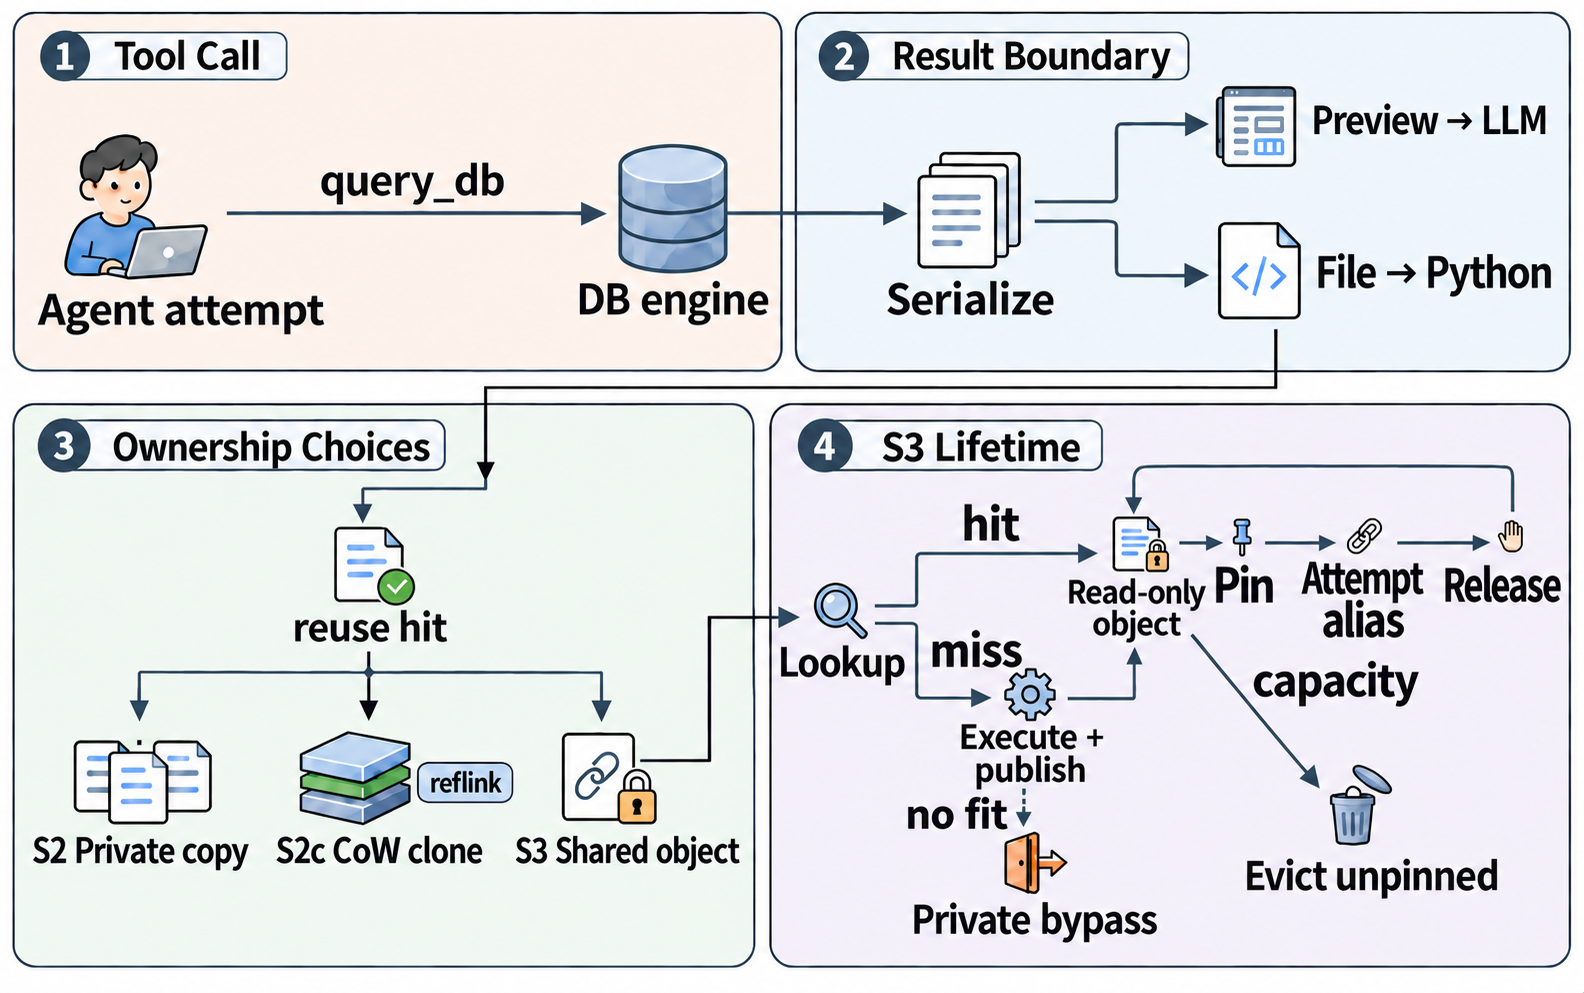
\includegraphics[width=\columnwidth]{figures/fig4a_ownership}}\\[3pt]
  \subcaptionbox{Footprint vs.\ $N$\label{fig:footN}}{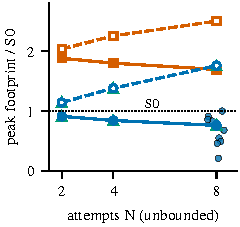
\includegraphics[height=1.45in]{figures/fig4b_footprint_N}}\hfill
  \subcaptionbox{Footprint vs.\ budget\label{fig:footB}}{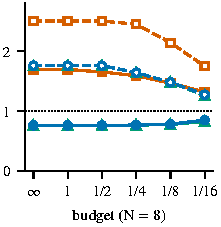
\includegraphics[height=1.45in]{figures/fig4c_footprint_budget}}\\[1pt]
  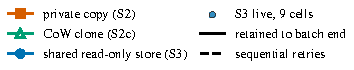
\includegraphics{figures/fig4_legend}
  \caption{Result ownership decides storage cost. (a) A \texttt{query\_db} result is serialized into an LLM preview and a file for Python. Only the file takes part in ownership. On a hit, S2 provides a private copy and S2c a reflink clone. S3 aliases one shared read-only object. SD is omitted because it changes execution but retains attempt-private serialization and files. Section~\ref{sec:designs} describes the lifetime of an S3 object. (b, c) Simulated peak footprint relative to no sharing (S0) on the assumption-based E-eval subset. Values are medians over the 52 tasks with nonzero S0 footprint (50 resamples). Panel (b) uses an unbounded budget and panel (c) uses $N=8$.
  Solid lines retain outputs to batch end, and dashed lines are sequential retries. Dots in (b) are live S3/S0 on the
  9 calibration cells with admitted spilled bytes ($N=8$, unbounded budget, median of 5 resamples, jittered). The
  simulator reproduces each cell.}
  \label{fig:ownership}
  \Description{Top: a four-region diagram. Region 1 shows an agent attempt calling query_db on a database engine. Region 2 shows the result serialized into a preview for the LLM and a file for Python. Region 3 shows three ownership choices on a reuse hit: a private copy, a copy-on-write clone, and a shared object. Region 4 shows the lifetime of a shared object: lookup, hit or miss with execute and publish, pin, attempt alias, release, eviction of unpinned objects under capacity pressure, and a private bypass when a result does not fit. Bottom: two line plots of peak footprint relative to no sharing. Private copies stay above 1, the shared store and clones stay near 0.76 to 0.91 when outputs are retained and between 1.14 and 1.76 for sequential retries.}
\end{figure}
